% == Cours de Java
% === Chapitre : Introduction

\begin{frame}{La machine virtuelle}
	\sigle{Java} a une approche mixte la \emph{machine virtuelle \sigle{Java}} (\sigle{JVM})  
\medskip
\begin{center}
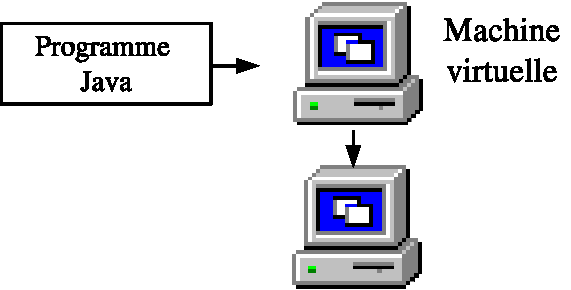
\includegraphics[scale=.8]{../img/java-jvm-jvm1} 
\end{center} 
\end{frame}

\full[bluepigment]{
	\begin{center}
		\Large\bf\color{azuremist}
		D'abord compil� \par ensuite interpr�t�
	\end{center}
}

\begin{frame}{La machine virtuelle}
\begin{center}
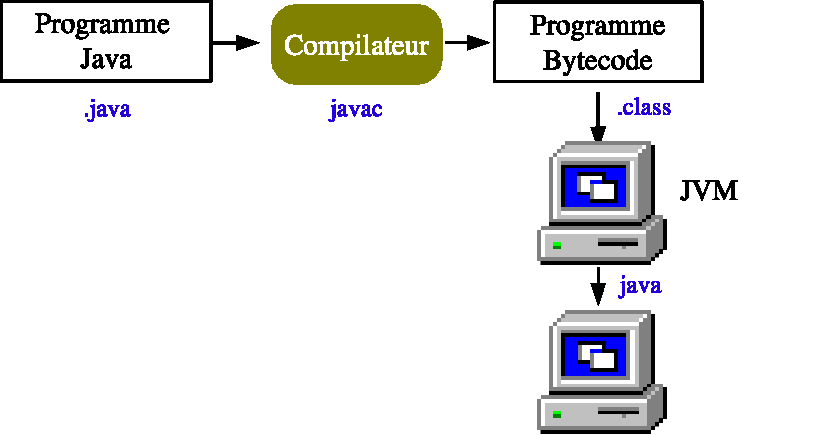
\includegraphics[scale=0.8]{../img/java-jvm-jvm2} 
\end{center}
\end{frame}

\imgfullw{../img/true-evolution.jpg}
	{\color{white}\textit{timeline \sigle{Java}}}
	{http://www.tshirthell.com/funny-shirts/true-evolution}

\begin{frame}[fragile]{Historique de \sigle{Java}}
\begin{itemize}
\item [\emph{92}] \sigle{SUN} cr�e \sigle{oak} (syst�mes embarqu�s).
\\Auteur: James Gosling
\item [\emph{94}] Adapt� � Internet gr�ce aux \emph{applets}. 
\\Devient \sigle{Java}
\item [\emph{96}] Premi�re version stable et gratuite de \sigle{JDK} 
\item [\emph{98}] Sortie de \sigle{Java 2}
\item [\emph{05}] Version \verb|1.5| de \sigle{Java 2}
\item [\emph{09}] \sigle{Oracle} rach�te \sigle{Sun} (et donc \sigle{Java})
\item [\emph{11}] Version \verb|1.7| (Java 7, en GPL)
\item [\emph{14}] Version \verb|1.8| (Java 8)
\end{itemize}
\end{frame}

\begin{frame}
	
\includegraphics[scale=.5]{../img/icon_39938.png}
	\begin{itemize}
		\item \sigle{Java} est-il install� sur ma machine ? 
		\item Puis-je commencer � �crire un programme \sigle{Java} ? 
		\item Qu'ai-je pris comme note ? 
	\end{itemize}
	\note[item]{Introduire les termes : JRE, JDK, ME, SE, EE}
\end{frame}
